\documentclass[a4paper,12pt]{article}
\usepackage[a4paper,landscape,margin=2cm]{geometry}
\usepackage{tikz}
\usetikzlibrary{arrows.meta, positioning}

\title{Server SVG Musei (Python + Flask)}
\author{Architettura e funzionamento}
\date{\today}

\begin{document}

\maketitle

\section*{1. Panoramica generale}

Il \textbf{Server SVG Musei} è un servizio Python basato su \textbf{Flask} che ha il compito di:
\begin{itemize}
  \item Generare dinamicamente \textbf{mappe SVG dei musei}.
  \item Recuperare la \textbf{struttura spaziale (layout)} da \textbf{MongoDB}.
  \item Recuperare i \textbf{dati logici del museo} (oggetti, connessioni) dal server Node.js.
  \item Combinare layout e dati logici per produrre una rappresentazione grafica coerente.
\end{itemize}

Il server non modifica dati: ha un ruolo \textbf{read-only e di rendering}.

\section*{2. Componenti principali}

\begin{itemize}
  \item \textbf{server.py (Flask)}: punto di ingresso HTTP, espone endpoint per ottenere SVG.
  \item \textbf{MongoDB (collection \texttt{musei\_layout})}: contiene i layout delle stanze per ciascun museo.
  \item \textbf{Server Node.js (openAPI)}: fornisce i dati logici del museo via REST.
  \item \textbf{model.py}: definisce le classi \texttt{Stanza} e \texttt{Oggetto}.
  \item \textbf{layout.py}: calcola corridoi e posizionamento spaziale delle stanze.
  \item \textbf{svg\_writer.py}: converte strutture interne in SVG finale.
\end{itemize}

\section*{3. Connessioni tra i componenti}

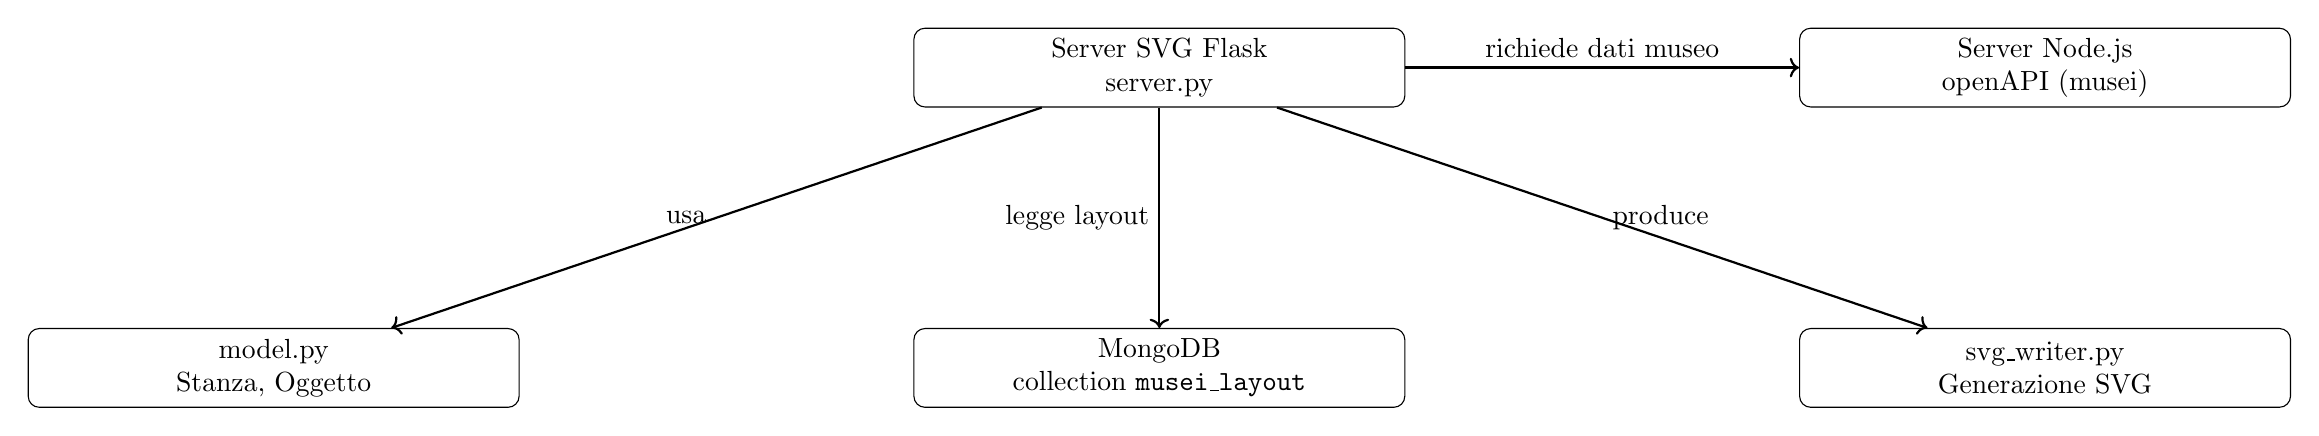
\begin{tikzpicture}[
  node distance=2.8cm and 5cm,
  box/.style={rectangle, draw, rounded corners, text width=6cm, align=center, minimum height=1cm}
]

\node[box] (flask) {Server SVG Flask\\server.py};
\node[box, below=of flask] (mongo) {MongoDB\\collection \texttt{musei\_layout}};
\node[box, right=of flask] (node) {Server Node.js\\openAPI (musei)};
\node[box, below left=of flask] (model) {model.py\\Stanza, Oggetto};
\node[box, below right=of flask] (svg) {svg\_writer.py\\Generazione SVG};

\draw[->, thick] (flask) -- (mongo) node[midway,left]{legge layout};
\draw[->, thick] (flask) -- (node) node[midway,above]{richiede dati museo};
\draw[->, thick] (flask) -- (model) node[midway,left]{usa};
\draw[->, thick] (flask) -- (svg) node[midway,right]{produce};

\end{tikzpicture}

\section*{4. Endpoint esposti}

Il server espone endpoint HTTP di sola lettura:

\begin{itemize}
  \item \texttt{/NomeMuseo}
  \item \texttt{/NomeMuseo/edge\_mode}
  \item \texttt{/NomeMuseo/edge\_mode/f1/f2}
\end{itemize}

\textbf{Risposta}: un documento \texttt{image/svg+xml} che rappresenta la mappa del museo.

\section*{5. Flusso di funzionamento}

\begin{enumerate}
  \item Il client richiede l'SVG di un museo.
  \item Il server Flask attende che il server Node sia online.
  \item Il layout del museo viene recuperato da MongoDB.
  \item I dati logici (oggetti, connessioni) vengono richiesti al server Node.
  \item Vengono istanziate le classi \texttt{Stanza} e \texttt{Oggetto}.
  \item Il layout viene calcolato (stanze + corridoi).
  \item Il risultato finale viene convertito in SVG.
\end{enumerate}

\section*{6. Dati gestiti}

\subsection*{6.1 Layout (MongoDB)}
Ogni documento layout contiene:
\begin{itemize}
  \item Identificatore del museo (\texttt{\_id}).
  \item Griglia di stanze con coordinate (\texttt{row}, \texttt{col}).
  \item Tipo della stanza (ingresso, uscita, bagno, servizio).
\end{itemize}

\subsection*{6.2 Dati museo (Node.js)}
Il server Node fornisce:
\begin{itemize}
  \item Nome e città del museo.
  \item Lista degli oggetti.
  \item Connessioni logiche tra oggetti.
\end{itemize}

\section*{7. Sicurezza e robustezza}

\begin{itemize}
  \item \textbf{API Key}: richiesta per comunicare con il server Node.
  \item \textbf{Timeout controllati}: evita blocchi su servizi non disponibili.
  \item \textbf{Attesa attiva all'avvio}: Flask parte solo quando Node è pronto.
  \item \textbf{HTTPS supportato}: comunicazione cifrata con il server Node.
\end{itemize}

\section*{8. Ruolo nel sistema complessivo}

Il server Python:
\begin{itemize}
  \item Non modifica dati persistenti.
  \item Non gestisce CRUD.
  \item È responsabile esclusivamente della \textbf{visualizzazione}.
  \item Separa nettamente \textbf{logica dei dati} e \textbf{rappresentazione grafica}.
\end{itemize}

\end{document}
